\documentclass[main.tex]{subfiles}
\begin{document}
Il s'agit de regarder la stabilité, la convergence vers un point d'équilibre. On se place dans le cas présent  en régime libre pour un système invariant, c'est à dire que $\dot{x} = f(x,u=0)$ et $y = g(x,u=0)$.\\


On pose $u=0$, car la stabilité et la dynamique du système sont des caractéristiques intrinsèques d'un système, donc indépendantes de l'entrée.\\

Pour étudier la stabilité, on se place dans le plan de phase. Celui-ci permet de situer les points d'équilibres et de vérifier la stabilité. Sa dimension est égale au nombre de variables d'état.

Ainsi, pour des systèmes du second ordre, on va avoir:
\[\begin{matrix}
x= \begin{pmatrix}x_1\\x_2\end{pmatrix} &\text{et}& f(x)=\begin{pmatrix}f_1(x)\\f_2(x)\end{pmatrix}
\end{matrix}\]
L'espace des phases devient alors ici un plan de phase dans lequel on va rechercher les trajectoires.

Dans la suite, on s'intéressera au cas de dimension deux pour positionner et comprendre le problème.

\section{Analyse qualitative du comportement}
Soit le système LTI obtenu à partir de la linéarisation autour d'un point d'équilibre $x_0$.\\
On dit que ce point d'équilibre est stable si c'est un point de convergence des trajectoire, ou instable si c'est un point de divergence des trajectoires.\\

On étudie donc le système autour de son point d'équilibre, en linéarisant son équation autour de ce point. On a donc l'équation:
\begin{align*}
\Aboxed{\delta \dot{x}&= A \delta x}\\
\text{où, } A&= \frac{\partial f(x)}{\partial x}|_{x=x_0} \text{	Jacobien de f en $x_0$}\\
\text{et, }\delta x &= x-x_0
\end{align*}

\begin{rem}
En N.L, la stabilité est associée aux points d'équilibres. Ainsi, un même système N.L peut avoir des points d'équilibres stables et instables.
  Cette approximation peux être également réalisée dans le cas d'un régime forcé:
  \[
    \begin{cases}
      \dot{x} = f(x,u)\\
      y = h(x,u)
    \end{cases}
  \]
  avec $f(\bar{x},\bar{u}) = 0$ et on alors:
  \[
    \begin{cases}
      f(\bar{x}+\delta x,\bar{u}+\delta u) = f(\bar{x},\bar{u}) + A. \delta x + B \delta u\\
      h(\bar{x}+\delta x,\bar{u}+\delta u) = h(\bar{x},\bar{u}) + C. \delta x + D \delta u
    \end{cases}
  \]
  Donc :
  \[
    \begin{cases}
      \delta \dot{x} = A. \delta x + B. \delta u \\
      \delta \dot{u} = C. \delta x + D. \delta u
  \end{cases}
  \]
\end{rem}
\emph{L'analyse qualitative de la stabilité est faite par linéarisation.} \\
\begin{prop}
La trajectoire pour une condition initiale $\delta x_0$ est solution de l'équation différentielle précédente, ie \[\delta x(t) = M exp(Jt)M^{-1}\delta x_0\] où J est la matrice diagonale ou de Jordan\footnotemark de A, la matrice d'évolution, et M la matrice de vecteurs propres tel que : $M^{-1}AM = J$.\\
\end{prop}
\footnote{cf UE421}
\subsection{Cas $\mathbb{R}$}
$J = \begin{pmatrix}
\lambda_1 &0 \\0&\lambda_2
\end{pmatrix}$ où $\lambda_1 \neq \lambda_2$\\
On pose le changement de variable $\delta z = M^{-1}\delta x$ : Base Modale.\\ Donc on a $\delta z_0 = M^{-1}\delta x_0$ comme valeur initiales, d'où :
\begin{align*}
\delta z_1(t) &= e^{\lambda_1t}\delta z_{01}\\
\delta z_2(t) &= e^{\lambda_2t}\delta z_{02}
\end{align*}
Ceci permet de tracer les trajectoires dans la base modale.\\

\begin{enumerate}

\item Dans le cas où  $\lambda_2 < \lambda_1 < 0$ ou $0 <  \lambda_1 < \lambda_2$, on obtient:
\begin{center}
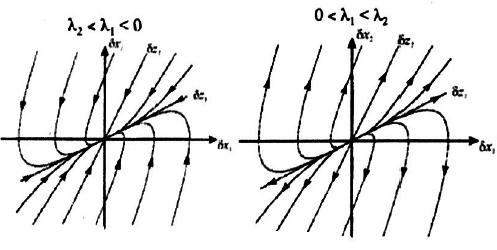
\includegraphics[scale=0.5]{1/graph3.png}
\end{center}
D'un coté on à la convergence plus rapide de $\delta z_2$ par rapport à $\delta z_1$ et de l'autre la divergence plus rapide de $\delta z_2$ par rapport à $\delta z_1$. On a un \emph{noeud} qui est donc soit stable soit instable. Et son \emph{index topologique vaut $+1$}\\

\item Dans le cas où  $\lambda_2 < 0 < \lambda_1 $, on obtient:
\begin{center}
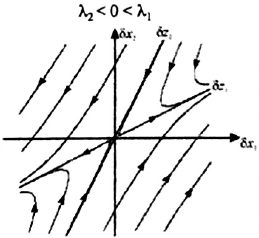
\includegraphics[scale=0.5]{1/graph4.png}
\end{center}
On est dans un cas instable et on a un point selle, d'index $-1$ \\


\item Dans le cas ou $\lambda_1 = 0$, on a:
\begin{align*}
\delta z_1 &= \delta z_{01}\\
\delta z_2 &= e^{\lambda t} \delta z_{02}
\end{align*}
d'où le graphique:
\begin{center}
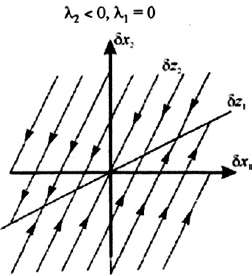
\includegraphics[scale=0.5]{1/graph6.png}
\end{center}
Il n'y a pas de point d'équilibre car A est non inversible ce qui implique que $\dot{x}=Ax \Rightarrow x=0$\\

\begin{rem}
Il n'y a pas de point d'équilibre d'après la définition $ \dot{x} = 0$ même si graphiquement on converge vers un point.
\end{rem}

\item Dans le cas où $\lambda_1 = \lambda_2 = \lambda$\\
Si $J = \begin{pmatrix}\lambda & 0 \\ 0 & \lambda\end{pmatrix}$ le sous espace propre est de dimension 2.\\
On a un point d'équilibre.


Si la dimension du sous espace propre est de 1, $J = \begin{pmatrix}\lambda & 1 \\ 0 & \lambda\end{pmatrix}$, donc :
\begin{align*}
\delta z_1 &= t e^{\lambda t} \delta z_{01} + e^{\lambda t} \delta z_{02}\\
\delta z_2 &= e^{\lambda t} \delta z_{02}
\end{align*}
\begin{center}
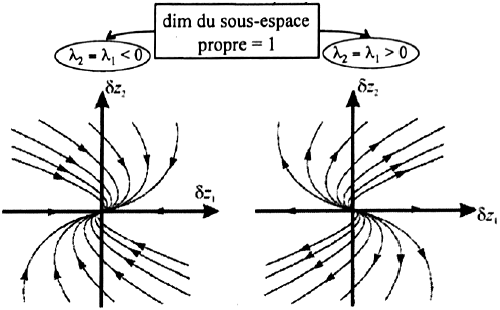
\includegraphics[scale=0.5]{1/graph5.png}
\end{center}

\end{enumerate}


\subsection{Cas $\mathbb{C}$}
 On a maintenant $\lambda_{1,2} = \alpha \pm j\beta$. On considère la représentation d'état : $\delta \dot{z_1} = M^{-1} \delta x$ tel que :
 \begin{align*}
 \delta \dot{z_1} &= \alpha \delta z_1 - \beta \delta z_2\\
 \delta \dot{z_2} &= \beta \delta z_1 + \alpha \delta z_2
 \intertext{On utilise les coordonnées polaires :}
 r = \sqrt{\delta z_1^2 + \delta z_2^2} &\text{ et, } \theta = arctan\left(\frac{\delta z_2}{\delta z_1}\right)
\intertext{on a donc :}
\dot{\theta} &= \beta\\
\dot{r} &= \alpha r
 \end{align*}
Ainsi, on obtient :
\[\left \{ \begin{matrix}
\theta(t) = \theta_0 + \beta t\\
r(t) = e^{\alpha t} r_0
\end{matrix}\right.\]

\begin{center}
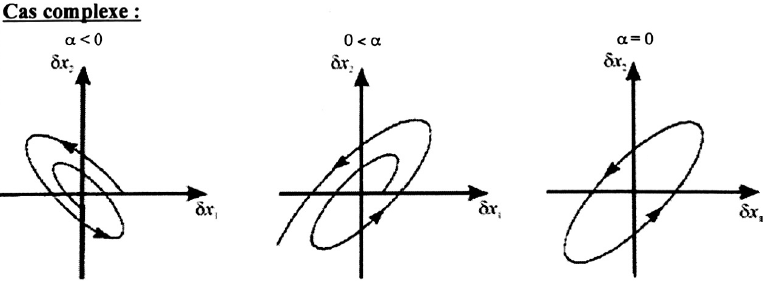
\includegraphics[scale=0.5]{1/graph7.png}
\end{center}
\[
  \begin{cases}
  \delta z_1(t) & = e^{\lambda t} \\
  \delta z_{10} + te^{\lambda t} \delta z_{20}\\
  \delta z_2(t) & = e^{\lambda t} \delta z_{20}
\end{cases}
\]
\nopagebreak[1]
\section{Cycle limite}
\begin{defin}
  Un système $\dot{x}=f(x)$ possède un \emph{cycle limite} $\mathcal{C}$ si il existe un intervalle de temps $[t_0,t_0+T]$ et $\forall x_0 \in \mathcal{C}$ tel que la trajectoire $\chi(t,x_0)$ soit solution de $\dot{x}=f(x)$ et avec $\chi(t_0,x_0)=x_0$et vérifie :
  \begin{itemize}
  \item $\chi(t,x_0) \in \mathcal{C}\quad \forall t\in[t_0,t_0+T[$
  \item $\chi(t_0+T,x_0) =x_0$
  \end{itemize}
\end{defin}


On considère un système oscillant, c'est à dire qu'il existe $T>0$ tel que $\forall t > 0$, $x(t+T) = x(t)$.\\
(On exclut cependant le cas $x(t)$ = constante).
\begin{rem}
  Un point d'équilibre peut être interpréter comme un cycle limite singleton $ \forall T\in\R$.
\end{rem}

\begin{prop}
  \begin{description}
  \item[Cycle limite stable]~\\
Pour toutes les conditions initiales appartenant au voisinage du cycle limite:
\[\exists t_0 > 0 \text{ et }T > 0 \text{ tel que } \forall t>t_0, \quad x(t+T) = x(t)\]
i.e. toute trajectoire dans un voisinage du cycle limite converge dans un temps fini vers le cycle limite.
\item[Cycle limite instable]~\\
Toutes les trajectoires divergent du cycle limite.\\
Pour toutes les CI n'appartenant pas au cycle limite, $ \exists t > 0 \text{ tel que} x(t) \notin \text{cycle limite} $.

\item[Cycle semi-stable]~\\
 Une partie des trajectoires converge et d'autres divergent du cycle limite.
\end{description}
\end{prop}


\begin{example}[Oscillateur de Van der Pol]
\[
  \begin{cases}
\dot{x_1} & = x_2\\ \dot{x_2} & = -x_1 + (1-x_ 1^2)x_2
\end{cases}
\]

Point d'équilibre $x^* =(0,0)$
\begin{rem}
Il n'existe pas de solution analytique aux équations de Van der Pol, mais numériquement on trouve un cycle limite stable.
\end{rem}

%\img{0.3}{3/2.png}

$\exists \epsilon$ tel que le cycle limite $\subset$ cercle de centre (0,0) et de rayon $\epsilon$ : stable au sens de Lagrange.\\

\end{example}

\begin{thm}[Index de Poincaré]~\\
  Dans le plan de phase (pour un système d'ordre 2) avec $N$ le nombre de noeuds, centre et foyer et $S$ le nombre de points selles.\\
  Si un cycle limite existe, les points d'équilibre que le cycle limite encercle sont tel que
  \[
\boxed{N =S +1}
  \]
\end{thm}
ce théorème s'utilise souvent sous sa forme contraposée:
\begin{corol}
  Si $N\neq S+1$ alors il n'existe pas de cycle limite.
\end{corol}

\begin{proof}~ \\
\begin{lemme}
  Soit une courbe du plan de phase alors l'index de la courbe est la somme des index des points d'équilibre contenu dans cette courbe.
\end{lemme}

À partir de cette proposition on peux démontrer le théorème de l'index de Poincaré, car le cycle limite $\mathcal{C}$ est solution de l'équation dynamique. l'index de $\mathcal{C}$ vaut +1. Ainsi le nombre de points d'équiliobre ayant l'index +1 doit être supérieur d'une unité à ceux dont l'index est -1
\end{proof}

\section{Théorème de Bendixon}

\begin{thm}
Soit le système du second ordre $\dot{x}=f(x)$ avec $f$ le champ de vecteurs tel que $f:D\rightarrow\R^2$ avec $D$ un ensemble simplement connexe (d'un seul tenant, non formé de la réunion d'ensemble disjoint, sans trous) de $\R^2$ ne contenant pas de point d'équilibre.
Si:
\begin{itemize}
\item $\exists x \in D$ tel que $\divv f(x) \neq 0$
\item $\divv f$ ne change pas de signe dans $D$
\end{itemize}
Alors $\dot{x}=f(x)$ n'a pas de cycle limite inclus dans $D$.
\end{thm}

\begin{proof}
Par l'absurde, soit $\Gamma = \{x\in D, x(t), 0 \leq t \leq T\}$ est un cycle limite.

$\forall x \in \Gamma$, $f(x)$ est tangent à $\Gamma$ tel que $f(x).n(x)=0$ où $n(x)$ est le vecteur normal de $\Gamma$ en $x$.

Suivant le théorème de Green,
\[ \oint_{\Gamma} f(x)n(x)dx = \iint_S \divv f(x)dS  \text{ donc } \iint_S \divv f(x)dS = 0
\]

Si $\exists x \in D$ tel que $\divv f(x) \neq 0$ et que $\div f$ ne change pas de signe dans $D$ (donc a fortiori dans $S\subset D$), on déduit de la continuité de l'opérateur $\divv f$ dans $D$ que $\iint_S \div f(x)dS \neq 0$ : contradictoire.

Ainsi, $D$ ne contient pas de cycle limite.
\end{proof}

\begin{example}
Soit le système NL du 2nd ordre $\ddot{x}(t) + \alpha \dot{x}(t) + g(x(t)) = 0$, avec $x(0) = x_0$ et $\dot{x}(0) = \dot{x}_0$ où $\alpha \neq 0$ et $g:\R \rightarrow \R$ continue avec $g(0)=0$. \\
Représentation d'état :
\[
  \begin{cases}
\dot{x}_1(t) & = x_2(t) = f_1(x)\\
  \dot{x}_2(t) & = - \alpha x_2(t) - g(x_1(t)) = f_2(x)
\end{cases}
\text{ avec } x_1(t) = x(t) \text{ et }x_2(t) = \dot{x}(t) \]

Calculons $\divv f = \derivp[f_1]{x_1} + \derivp[f_2]{x_2} = -\alpha$.

$\divv f \neq 0$ et ne change pas de signe donc ce système ne comporte pas de cycle limite $(D=\R^2)$.
\end{example}
\section{Théorème de Poincaré-Bendixon}
\begin{defin}
  \begin{itemize}
  \item Un ensemble $\mathcal{M}\subset \mathcal{D}$ est dit \emph{positivement
      invariant} du système $\Sigma$ si
  \[\chi_t(\mathcal{M}) \subseteq \mathcal{M} , \forall t \ge 0\]
\item   Si la propriété est vraie $\forall t\le 0 $ l'ensembles est \emph{négativement invariant}.
  \item Si la propriété est vraie $\forall t\in \R$ . l'ensembles est \emph{invariant}
\end{itemize}
\end{defin}
\begin{rem}
  Un ensemble invariant est un fermé de $\R^n$.
\end{rem}

\begin{rem}
  Un cycle limite stable ou semi-stable est un cas particulier d'un ensemble invariant. Cet ensemble est un \emph{attracteur} et  ne peut avoir qu'un comportement périodique.
\end{rem}

\begin{defin}
  Un \emph{attracteur} est un ensemble invariant fermé $\mathcal{M} \subset \mathcal{D}$ du système $\Sigma$, si il existe un voisinage $\mathcal{N}$ de $\mathcal{M}$ tel que
  \[
    \forall x\in \mathcal{N}, \text{ et } \chi_t(x) \in \mathcal{N}, \forall t \ge 0 , \chi_t(x) \xrightarrow[t\to\infty]{} \mathcal{M}^t
  \]
\end{defin}
\begin{rem}
  Physiquement\footnote{\emph{sic.}} un attracteur est un fermé borné (compact)
\end{rem}

\begin{thm}
Soient le système du 2nd ordre $\dot{x}=f(x)$ et $O_{x_0}^+$ une trajectoire positive, i.e $O_{x_0}^+ = \{ x \in D, x = S(t,x_0), t \geq 0\}$ où $S(.,x) : \R \rightarrow D$ définit une solution de $\dot{x}=f(x)$ pour une trajectoire passant par $x$, avec un ensemble limite $\omega(x_0)$ i.e. \footnotemark $\omega(x_0) = \bigcap_{t \geq 0} \overline{O_{x_0}^+}$ \\

Si $\omega(x_0)$ est compact et ne contient pas de point d'équilibre, alors la limite ne peut être qu'un cycle limite.\\
\end{thm}
\footnote{adhérence = plus petit fermé contenant l'ensemble}

Interprétation :

Dans le cas du 2nd ordre, si on a une convergence des trajectoires vers un compact (fermé borné de $\R^2$) qui ne contient pas de point d'équilibre, alors la limite ne peut être qu'un cycle limite.\\

\begin{prop}
  \begin{itemize}
  \item $\omega_0$ définit un ensemble positivement invariant.
  \item Dans $\R^2$ le seul attracteur possible est un cycle limite.
  \item Si la trajectoire converge vers un ensemble alors on a les cas possibles:
    \begin{itemize}
    \item C'est un ensemble de points d'équilibres.
    \item C'est un cycle limite.
    \item La trajectoire est un cycle limite.
    \end{itemize}
  \end{itemize}
\end{prop}

Exemple 1 :
\begin{align*}
\dot{x} & =
          \begin{bmatrix}
-1 & 10 \\-100 & -1
\end{bmatrix} x = A_1x\\
\dot{x} & =
          \begin{bmatrix}
-1 & 100 \\ -10 & -1
\end{bmatrix}x = A_2x
\quad \text{v.p. } \lambda_{1,2} = -1 \pm j31,62
\end{align*}

Les deux systèmes sont stables

Stabilité locale mais le système est instable globalement.\\

Important : l'analyse faite par linéarisation donne uniquement une information sur la stabilité locale et non globale.\\

Exemple 2 :
\begin{align*}
\dot{x} & =
          \begin{bmatrix}
1 &- 10\\100 & 1 x
\end{bmatrix}
= A_1x \\
\dot{x} & =
          \begin{bmatrix}
1 & -100\\10 & 1
\end{bmatrix}
x = A_2x \quad \text{v.p. } \lambda_{1,2} = -1 \pm j31,62
\end{align*}

Les deux systèmes sont instables.

En choisissant bien la permutation, on rend le système global stable.

\paragraph{Conclusion} l'analyse de la stabilité par linéarisation ne donne pas une CNS de stabilité des systèmes non linéaires (point d'équilibre), d'où l'importance de définir un autre moyen d'analyse. \\

\begin{rem}
Il existe d'autres méthodes pour tracer les trajectoires dans le plan de phase.
\end{rem}

\begin{exemple}[Élimination du temps]
\noindent Méthode explicite :
\[
  \begin{cases}
x_1(t) & = x_0 \cos t + \dot{x}_0 \sin t\\x_2(t) & = -x_0 \sin t + x_0 \cos t
\end{cases}
\]

\[x_1^2(t) + x_2^2(t) = x_0^2 + \dot{x}_0^2 \]
On a éliminé le temps mais c'est assez \emph{spicifique} à la représentation d'état.

\noindent Méthode implicite :
\[ \dot{x} =
  \begin{bmatrix}
0 & 1 \\ 1 & 0
\end{bmatrix}
x \text{ donc }
  \begin{cases}
  \dd{x_1}{t} & = x_2\\ \dd{x_2}{t} & = -x_1
\end{cases}
\]
\[dt = \frac{dx_1}{x_2} = -\frac{dx_2}{x_1}\]
\[x_1dx_1 = -x_2dx_2 \text{ donc } x_1^2 + x_2^2 = x_{20}^2 + x_{10}^2\]
\end{exemple}
\end{document}

%%% Local Variables:
%%% mode: latex
%%% TeX-master: "main"
%%% End:
